\documentclass{bioinfo}
\copyrightyear{2016} \pubyear{2016}

\access{Advance Access Publication Date: Day Month Year}
\appnotes{Application Note}

\usepackage{url}

\begin{document}
\firstpage{1}

\subtitle{Application Note}

\title[Indel Historian: phylogenetic ancestral reconstruction]{Indel Historian: fast and accurate ancestral sequence reconstruction}
\author[Ian Holmes]{Ian Holmes$^{\text{\sfb 1}*}$}
\address{$^{\text{\sf 1}}$Department of Bioengineering, University of California, Berkeley, 94703, USA.}

\corresp{$^\ast$To whom correspondence should be addressed.}

\history{Received on XXXXX } %; revised on XXXXX; accepted on XXXXX}

\editor{Associate Editor: XXXXXXX}

\abstract{
{\bf Motivation.}
Reconstruction of indel histories and ancestral sequences is a specialized variation of multiple sequence alignment.
%The best alignment tools for ancestral reconstruction
%are not necessarily those that agree most closely with benchmark datasets based on 3D structure alignments.
In previously published simulations,
the alignment tool ProtPal (based on a statistical phylogenetic model combining indel and substitution processes)
reconstructed indel histories more accurately than other tools,
but has proven too slow for practical use.
{\bf Results.}
Indel Historian combines an efficient reimplementation of the ProtPal algorithm with performance-improving heuristics from other alignment tools.
Simulation results on fidelity of ancestral sequence reconstruction,
along with evaluations on the structurally-informed datasets BAliBase and PREFAB, are reported.
{\bf Availability and Implementation.}
Indel Historian is available at \url{https://github.com/ihh/indelhistorian} under the Creative Commons Attribution 3.0 US license.
{\bf Contact.}
Ian Holmes {\tt ihholmes+indelhistorian@gmail.com}.
{\bf Supplementary Information.}
None.
}

\maketitle

\section{Introduction}

Multiple alignments are used for several purposes in bioinformatics,
only one of which is homology-directed protein structure prediction,
yet structurally-derived alignments have tended to dominate benchmarks.
There is evidence that for evolutionary applications, such as reconstructing trees or ancestral sequences,
different alignment tools (along with different tool-assessment metrics) might be preferable.
Aligners that are optimized for detecting structural homology may not do so well at recovering information about substitution rates,
whereas explicit statistical models of the sequence evolution process may do a better job at estimating these parameters.

Empirical studies suggest that, for the purposes of estimating
molecular evolutionary parameters---such as indel rates \citep{Westesson2012-zg},
dN/dS ratios \citep{Redelings2014},
or trees \citep{LoytynojaGoldman2008}---it is advantageous to use a statistical model of evolution
and to treat alignment rigorously as a ``missing data'' problem.
One possible explanation is that, for protein structure prediction,
detailed reconstruction of indel histories in fast-evolving regions (such as loops) is unnecessary
(as structurally homologous loops can simply be aligned),
whereas evolutionary analyses can make use of this information.

The benchmarks commonly used to evaluate aligners use accuracy scores
(such as SPS, TCS, AMA, and the Cline shift score)
which quantify the number of correctly aligned residues
compared to a dataset of structurally-informed reference alignments \citep{ThompsonEtAl2005}.
Techniques that score highly in these tests include using Bayesian decision theory to maximize the expected
alignment accuracy \citep{NotredameEtAl2000,DoEtAl2005,SchwartzPachter2007,BradleyEtAl2009}
and fine-tuning the alignment scoring function for contextual details, such as the reduced propensity for indels in
hydrophobic protein regions \citep{Edgar2004b,KatohEtAl2005,LarkinEtAl2007}.
Aligners have also been tuned for performance by optimizing rate-limiting steps
uch as all-versus-all pairwise sequence comparison \citep{Edgar2004b,BradleyEtAl2009}.

In a previous study, we sought to quantify systematic biases introduced into the
estimation of indel rates \citep{Westesson2012-zg},
using the evolution simulator indel-Seq-Gen \citep{StropeEtAl2009}.
The ProtPal program \citep{Westesson2012-zg}, which models indel evolution using 
transducers---finite-state machines which can be multiplied together like substitution matrices \citep{BouchardCote2013}---introduced
the least biases of the tools evaluated (RMS error 25\% for insertion rates and 25\% for deletion rates),
followed by PRANK (RMS error 40\% for insertions, 34\% for deletions) and then a MUSCLE-based workflow (45\%, 37\%).
Biases were substantially worse at higher indel rates: e.g. for the highest simulated insertion rate of 0.08 insertions/substitution,
the RMS estimation errors were 43\% (ProtPal), 64\% (PRANK) and 74\% (MUSCLE).

Unfortunately, the implementation of ProtPal published with that benchmark was too slow
for practical use.
Here, we present a clean reimplementation of the algorithm underlying ProtPal
in a new tool, Indel Historian.
We also report an assessment of the alignment accuracy
on structurally-derived benchmarks,
complementing the above-described evolution-oriented simulation experiments.

\begin{methods}
\section{Methods}

Indel Historian combines established algorithms from several sources.
Like ProtPal, Indel Historian progressively climbs a tree from tips to root,
building an ancestral sequence profile that includes suboptimal alignments \citep{LeeGrassoSharlow2002,Westesson2012-zg}
using a time-dependent evolutionary model \citep{RivasEddy2015}.
The guide tree is found by neighbor-joining % \citep{SaitouNei87}
on a guide alignment constructed from the all-vs-all pairwise alignment graph,
or from a sparse random connected subgraph \citep{BradleyEtAl2009}.
The guide alignment, which can also be supplied by another tool,
can optionally constrain the progressive reconstruction,
which is followed by iterative refinement \citep{HolmesBruno2001,Edgar2004b}.
Indel Historian also implements the phylogenetic EM algorithm for continuous-time Markov chains \citep{HolmesRubin2002},
so substitution and indel rates can be estimated directly from sequence data,
summing over the most probable alignments.

\end{methods}

\section{Results and Discussion}

\begin{figure}
  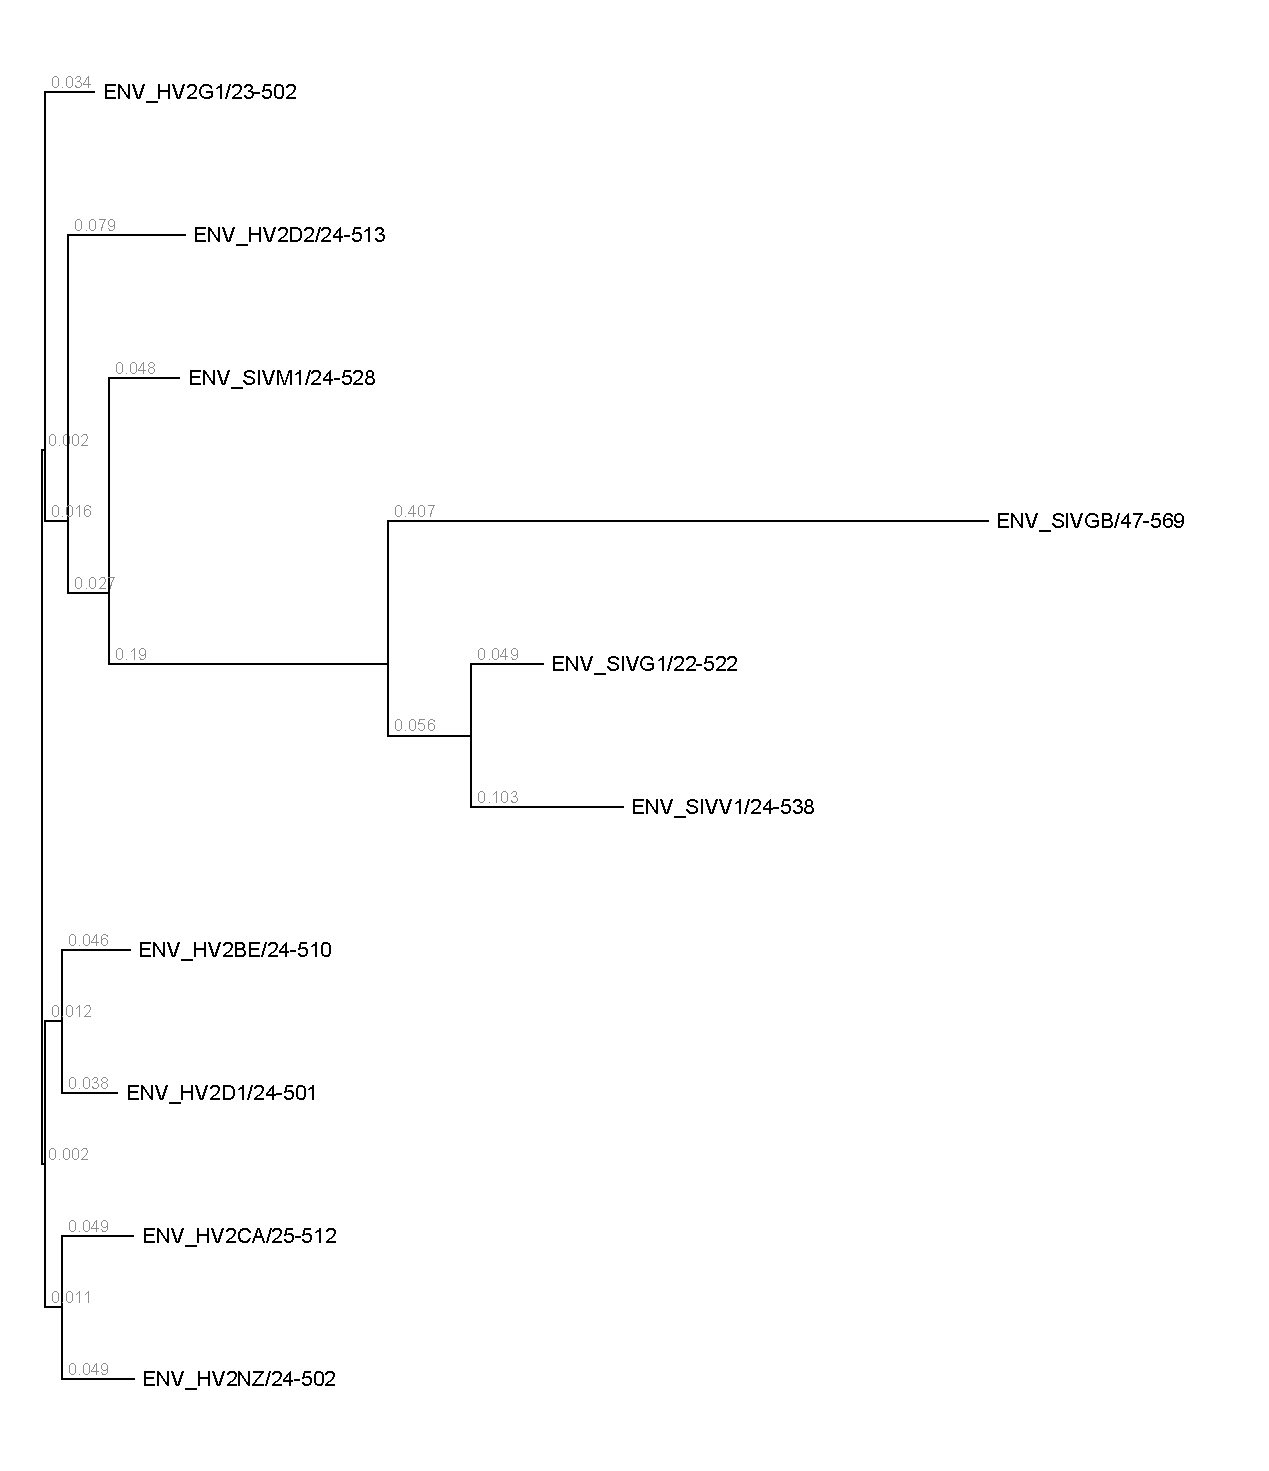
\includegraphics[width=\columnwidth]{gp120tree.pdf}
  \caption{
    Tree of HIV and SIV GP120 domains that was used for the simulation benchmark.
  }
\end{figure}

\begin{table}
  \begin{tabular}{r|r}
    & RMS error \\
    \hline
True alignment & \\
Indel Historian & \\
PRANK & \\
ProbCons & \\
MUSCLE & \\
  \end{tabular}
  \caption{
    Comparison of Indel Historian to other alignment programs on a simulation benchmark
    using datasets generated by indel-Seq-Gen \citep{StropeEtAl2009}
    with parameters mimicking an alignment of HIV GP120 domains.
  }
\end{table}

We first performed a simulation benchmark to assess Indel Historian's ability to reconstruct evolutionary parameters,
compared to other tools.
We based the simulation parameters on the evolutionary profile of the HIV GP120 envelope domain, as follows.
We started with an alignment of ten GP120 domains from HIV and SIV and estimated a tree from this alignment (Figure~1).
%The resulting tree has three branches that are over 0.1 substitutions/site in length (the relevant branch lengths are 0.10, 0.19, and 0.41).
%The remaining branch lengths were all under 0.1 subs/site; the median branch length was 0.046 subs/site.
We used the tree to estimate the indel rates for the alignment, and converted these to indel-Seq-Gen's parameter format.
To one significant figure, the probability of opening an indel at any given site on a unit-length branch is $p=0.3$, and the sequence length is 500 amino acids.

We then simulated 100 different alignments under these conditions, using indel-Seq-Gen, and attempted to estimate indel rates
(a) from the true alignment; (b) using alignments or reconstructions created by ProbCons, MUSCLE, PRANK, and Indel Historian.
In each case, we estimated insertion and deletion rates $(\hat{\lambda},\hat{\mu})$ and computed relative errors $(\frac{\hat{\lambda}-\lambda}{\lambda},\frac{\hat{\mu}-\mu}{\mu})$
compared to the true indel rates ($\lambda = \mu = \log(1-p)$).

The RMS (root mean square) of these errors are reported in Table~1.
Note that even perfect knowledge of the true alignment does not guarantee perfect reconstruction of the underlying indel rate parameters,
due to the possibility of indel events that are not directly observable (for example, when multiple indel events overlap on the same branch,
they will generally be conflated into a single event by the inference algorithm).

\begin{table}
  \begin{tabular}{r|rr|rr}
    & \multicolumn{2}{c|}{BAliBase 3.0} & \multicolumn{2}{c}{PREFAB 4} \\
    & Mean SPS & Mean TCS & Mean SPS & Mean TCS \\
    \hline
Indel Historian & 0.82 & 0.50 & 0.60 & 0.60 \\
CLUSTALW & 0.79 & 0.45 & 0.62 & 0.62 \\
PRANK & 0.73 & 0.35 & 0.51 & 0.51 \\
MAFFT & 0.87 & 0.61 & 0.69 & 0.69 \\
ProbCons & 0.88 & 0.62 & 0.72 & 0.72 \\
MUSCLE & 0.89 & 0.64 & 0.73 & 0.73
  \end{tabular}
  \caption{
    Comparison of Indel Historian to other alignment programs using standard benchmarks
    and the SPS/TCS scores \citep{ThompsonEtAl2005}.
    Average runtime per alignment was 55s for BAliBase and 39s for PREFAB (4 GHz Intel Core i7).
    Data for CLUSTALW, PRANK (+F option, CLUSTALW tree), MAFFT (v6.603), ProbCons (v1.12) and MUSCLE (version 4.0) are from {\tt http://drive5.com/bench/} \citep{Edgar2010}.
  }
\end{table}

Table~2 summarizes an evaluation of Indel Historian
on the BAliBase and PREFAB benchmarks,
compiled partially or wholly using 3D structural alignments.

In general, Indel Historian performs better on these structure-derived benchmarks than PRANK,
which also performs ancestral reconstruction \citep{LoytynojaGoldman2008},
and is the second-most accurate after ProtPal at estimating indel rates \citep{Westesson2012-zg}.
Compared to leading protein aligners that do not attempt ancestral reconstruction,
Indel Historian outperforms CLUSTALW \citep{LarkinEtAl2007} on BaliBase3, but not MUSCLE \citep{Edgar2004b},
ProbCons \citep{DoEtAl2005}, MAFFT \citep{KatohEtAl2005}, or CLUSTALW on PREFAB (though it is close).

\begin{table}
  \begin{tabular}{r|rr}
    & \multicolumn{2}{c}{Average run time per alignment} \\
 & Simulation & BAliBase 3 \\
    \hline
Indel Historian & & 55s \\
PRANK & & 519s \\
MUSCLE & & 1.9s \\
\end{tabular}
\caption{
    Comparison of runtimes of Indel Historian, PRANK and MUSCLE on the simulation benchmark and the BAliBase 3 benchmark.
  }
\end{table}

The results for the programs other than Indel Historian in Table~2 were taken from {\tt http://drive5.com/bench/} \citep{Edgar2010}.
To make a direct comparison of runtimes, we re-ran the benchmarks for PRANK and MUSCLE on the same machine as the Indel Historian benchmark.
These runtimes are summarized in Table~3: Indel Historian is an order of magnitude slower than MUSCLE, but an order of magnitude faster than PRANK.

We did not benchmark MCMC approaches
such as BaliPhy \citep{Redelings2014}, StatAlign \citep{NovakEtAl2008} or HandAlign \citep{WestessonBarquistHolmes2012}.
These are expected to be more accurate, but generally take much longer.
MCMC samplers may be usefully supplemented by decision-theoretic approaches to summarize a sampling run \citep{HermanEtAl2015}.
Other potential ways to improve accuracy include position-specific gap penalties, as used by MUSCLE \citep{Edgar2004b} and MAFFT \citep{KatohEtAl2005},
and explicit modeling of tandem duplications \citep{SzalkowskiAnisimova2013}.
Incorporating additional data such as structural annotations may further improve alignments \citep{HermanEtAl2014}.

% The best-performing method MUSCLE introduces heuristics into its scoring scheme
% that improve accuracy.
% 
% It is harder to incorporate these sorts of modifications into a rigorous phylogenetic model
% primarily because they violate the assumption of independence
% between indel and substitution processes
% that most such models rely on
% 
% Comparison to MCMC tools
% BaliPhy \citep{RedelingsSuchard2005,RedelingsSuchard2007,Redelings2014},
% StatAlign \citep{NovakEtAl2008,HermanEtAl2014},
% HandAlign \citep{WestessonBarquistHolmes2012}
% 
% Decision theory may also be useful to produce consensus alignments summarizing an MCMC run \citep{HermanEtAl2015}



\section{Availability}

Indel Historian is available at \url{https://github.com/ihh/indelhistorian} under the Creative Commons Attribution 3.0 US license. It is written in C++11, and compiles on a POSIX system with Clang (v.6.1.0). It requires the GNU Scientific Software library (libgsl), the ZLib compression library (libz), and the Boost C++ library.

\section*{Acknowledgements}

Indel Historian includes code from Ivan Vashchaev (gason), Heng Li (kseq), % Rafael Baptista (stacktrace), David Robert Nadeau (memsize), Roger Pate (string escaping), Konrad Rudolph (index sort),
and the StackOverflow community.

\section*{Funding}

This work has been supported by NHGRI grant R01-HG004483.

\bibliographystyle{natbib}
%\bibliographystyle{bioinformatics}
%\bibliographystyle{achemnat}
%\bibliographystyle{plainnat}
%\bibliographystyle{abbrv}
%
%\bibliographystyle{plain}
%
%\bibliography{Document}


\bibliography{references}
\end{document}
